\section{System architecture}
\label{sec:sysarch}

\subsection{Top level}

\begin{figure}
  \centering
  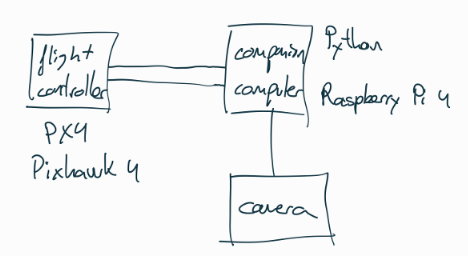
\includegraphics[keepaspectratio]{img/toplevel-sysarch.png}
  \caption{Top level diagram of the hardware/software interactions \todo[inline]{Draft, add QGC}}\label{fig:toplevel}
\end{figure}

The purpose of the Dronecontrol application is to be able to direct the movement of a \gls{uav} through the analysis of the images taken by a camera.
Since the processing power needed to work with the images recorded is superior to that offered by the autopilot flight controller it becomes necessary the use of an additional companion computer that will control the camera and employ machine learning to extract useful features from the images, as well as transform those features into movement directives for the vehicle.

A top level diagram of the individual parts that comprise the system is shown in Figure~\ref{fig:toplevel}. The main elements are the flight controller, that will run the PX4 autopilot \ref{subsec:px4}, the companion computer, that will run the developed application, and the camera, which provides the images.
The flight controller interfaces directly with the companion computer using the \gls{mavlink} protocol described in Section~\ref{subsec:mavlink}, either through a wireless radio link or a cabled serial connection between the two.
The camera is connected to the companion computer through a cable into an USB port on the computer.
Typically, the type of connection between the flight controller and the computer depends on the desired setup for the system so in the case where the camera, and therefore the companion computer, flies onboard the vehicle it is most convenient to use a direct wire connection between the two, as it provides a faster and more stable link. 
This onboard configuration is further detailed in Section~\ref{subsec:offboard}.
On the other hand, in the case where the companion computer will be acting more like a ground station on an offboard configuration it becomes strictly necessary to communicate with the flight controller through a wireless connection. For this purpose, a pair of telemetry radios provided with the Development Kit of the Holybro X500 (\ref{subsec:pixhawk}) are used. The complete setup requiered for this configuration is described in Section~\ref{subsec:onboard}.

In this project, the flight controller is driven by the PX4 software (\ref{subsec:px4}) and the hardware employed is optimized for this flight stack.
PX4 uses sensors to determine the vehicle state, which is needed for stabilization and to enable autonomous control.
It minimally requires a gyroscope, accelerometer, magnetometer (compass) and barometer.
A GPS or other positioning system is needed to enable all automatic flight modes, and some assisted ones.
PX4 uses outputs to control motor speed, flight surfaces like ailerons and flaps, camera triggers, parachutes, grippers, and many other types of payloads.
Many PX4 drones use brushless motors that are driven by the flight controller via an Electronic Speed Controller (ESC).
The ESC converts a signal from the flight controller to an appropriate level of power delivered to the motor.
PX4 drones are mostly commonly powered from Lithium-Polymer (LiPo) batteries.
The battery is typically connected to the system using a Power Module or Power Management Board, 
which provide separate power for the flight controller and to the ESCs for the motors.
A Radio Control (RC) system is used to manually control the vehicle.
It consists of a remote control unit that uses a transmitter to communicate stick/control positions with a receiver based on the vehicle.
Some RC systems can additionally receive telemetry information back from the autopilot.
Telemetry Radios can provide a wireless MAVLink connection between a ground control station and a vehicle running PX4.
This makes it possible to tune parameters while a vehicle is in flight, inspect telemetry in real-time, change a mission on the fly, etc.

On an actual UAV, the PX4 software runs on a dedicated piece of hardware like the Pixhawk 4 flight controller described in Section~\ref{subsec:pixhawk} that includes all the minimal required sensors for flight as well as interfaces to connect additional actuators and I/O systems (RC, telemetry radio, etc).
However, it is also possible to simulate this hardware on a standard Linux system by building the PX4 source code on a computer with this operating system.
This process is described in the development environment section (\ref{sec:devenv}).

The Dronecontrol application that runs on the companion computer has been developed using the Python programming language \footnote{\url{https://www.python.org/}}.
It offers good advantages for a project of this characteristics because of its high-level,
easy-to-use syntax, that usually results in a smaller code base than other comparable languages for small projects, its versatility and support for object-oriented programming. 
Most importantly, Python is widely used and its official package manager \verb|pip| greatly simplifies the use of external libraries and which gathers in its package index \footnote{\url{https://pypi.org/}} thousands of standard utilities,
including many machine learning and image processing projects and all the required libraries for interacting with PX4 through the MAVLink protocol (MavSDK).
As it is an interpreted language, it can run easily in any system with Python installed without the need to compile separate binaries for different operating systems.

The next sections explore deeper into the differences between the two configurations mentioned before: offboard computer (or ground station) and onboard computer.

\subsection{Offboard computer configuration}
\label{subsec:offboard}

The offboard configuration allows the flight controller to communicate and receive orders from a companion computer that is not physically connected to its hardware but that can instead stay on ground while the vehicle flies.
This has the advantage that it permits a simpler configuration, without having to be concerned with low-level hardware interactions between the two systems or powering of the companion computer while in flight, as well as allowing the use of a more powerful computer for image processing.
However, it also requires that the camera stays connected to computer on the ground so it cannot use images from the perspective of the drone in flight which limits the real-world applications of the system.
Other configurations involving a direct connection from a camera to the flight controller and the transmission of its images wirelessly to the companion computer through mavlink for processing can be feasible with the current technology but fall out of the scope of this project.

The wireless link is established in this instance through a pair of telemetry radios that connect to a telemetry port on the flight controller and to a USB port in the companion computer, respectively.
Since the Pixhawk 4 is configured by default to used its \verb|TELEM1| port for this purpose, no additional configuration is needed when using that port.
In the companion computer, applications like the QGRoundControl \footnote{\url{http://qgroundcontrol.com/}} ground station software which is part of the Dronecode Project are able to detect automatically a telemetry radio inserted into any of the USB ports of the host computer.
Additionally, other applications using the MavSDK (\ref{subsec:mavlink}) library can establish connection specifying the baudrate and the USB serial port address, usually something similar to \verb|/dev/ttyUSB0| on Linux and \verb|COM#| on Windows.

The radio used for the physical tests in this project is the Holybro SiK Telemetry Radio \footnote{\url{http://www.holybro.com/product/transceiver-telemetry-radio-v3/}}.
It is a small, light and inexpensive open source radio platform that typically allows ranges of better than 300m “out of the box” (the range can be extended to several kilometres with the use of a patch antenna on the ground).
The radios are offered either as 915Mhz (Europe) or 433Mhz (US) so they can be used in different regions and comply with the regulations for frequency, hopping channels and power levels.
They offer 2-way full-duplex communication through an adaptive TDM UART interface and their antenna allows for an adjustable 100-mW-maximum output power and -117 dBm receive sensitivity.
The link is established by default with a baudrate of 57600 (max bits per second on a serial channel) and it can provide air data rates of up to 250 kbps.

\todo[inline]{Images of the radios}
\todo[inline]{Images of the flight controller}
\todo[inline]{Connection diagram / pictures}

\subsection{Onboard computer configuration}
\label{subsec:onboard}

The second way of configuring the interaction between the flight controller and the companion computer consists of integrating both together on board the \gls{uav}.
In this case, the connection is done through a direct cable between the serial port in the flight controller and a USB port in the companion computer.
The camera will then be connected via cable as well to the companion computer and oriented in the vehicle in a way that allows for the best possible perspective during flight.
This configuration makes it possible to develop new control solutions based on images taken directly from the vehicle and that reflect the trajectory that it follows.
Therefore, it becomes possible to adjust the control loop based on previous reactions of the vehicle to commands and maintain a feedback loop for a more stable guidance.

Since the computer running the visual processing algorithm now has to fly on board the vehicle, it becomes specially important to make a good choice when selecting hardware.
To be able to take into the air, the computer has to be light enough that its weight can be lifted by the propellers while maintaining an adequate battery autonomy, but also powerful enough that the processor can handle the computer vision algorithms required to extract the necessary features from the images taken from the onboard camera that are to be feed to the control loop.

\begin{figure}
  \centering
  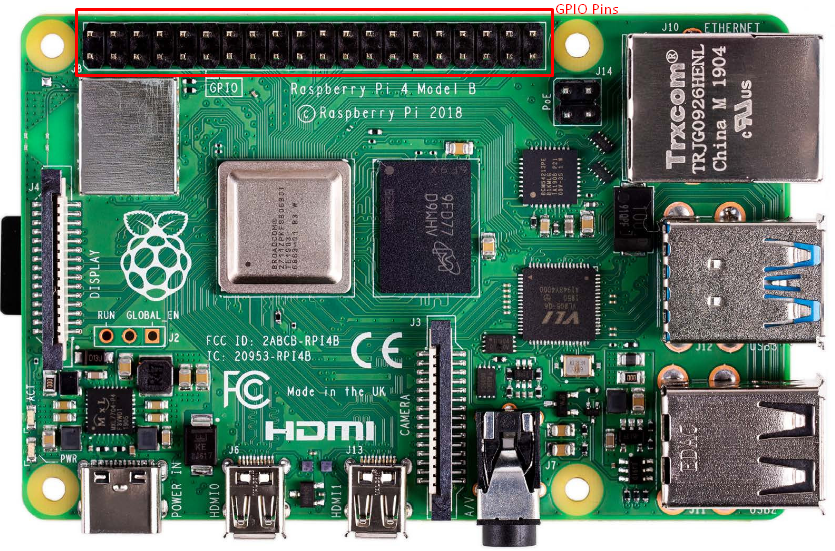
\includegraphics[width=\textwidth,keepaspectratio]{img/rpi4.png}
  \caption{The Raspberry Pi 4 microcomputer, with its 40-pin GPIO header marked in red}\label{fig:rpi4}
\end{figure}
\todo[inline]{Add pinout figure}
The Raspberry Pi 4 model chosen for this project and shown in Figure~\ref{fig:rpi4} is one of the most popular small computers available in the market at the time and it is widely use in all kinds of robotics projects both for education and hobbyists.
One of the most important advantages of using such a platform is the easy access to a great amount of manuals, guides and other support available online.
In addition, the Raspberry's officially supported operating system, called Raspberry Pi OS, is a Debian-based version of Unix optimized for its ARM microcontroller, which simplifies the process of moving from an Ubuntu test environment into real flight experiments.
Since this computer is designed to be easy to integrate with hardware projects it includes a 40-pin GPIO header (marked in red in Figure~\ref{fig:rpi4}) that can be programmed for connecting to any number of external devices.

The Raspberry Pi is powered by a 5V input that can be provided either from its USB-C port or through one of two pins in the header dedicated to this (marked as DC 5v power on Figure~\ref{fig:pinout}.
In the case of the particular vehicle build used in this project, the power management board used (the Holybro PM07 \footnote{\url{http://www.holybro.com/product/pixhawk-4-power-module-pm07/}}) also provides 5V to the flight controller, as well as powering the ESCs to the motors, and counts with two power outputs so one of them can be connected to the flight controller's \verb|POWER1| port and the other to the Raspberry Pi's pins through a custom-made connector.
\todo[inline]{Power management: more about this when it works}

In regards to the camera that will fly onboard the vehicle, there are many possibilities to chose from.
The most important characteristics that should be looked for are a small weight and simple plug-and-play interaction with the onboard computer.
For the tests carried out and detailed in Section~\ref{chap:validation} a Logitech 1080p webcam \todo{Exact model and link} has been used.
Since the frame of the Holybro X500 is not prepared by default to include an onboard camera, it became necessary to design a support to hang from the central rods of the vehicle frame where the camera could be attached securely during flight.
\todo[inline]{Pictures and 3D model}

\begin{figure}
  \centering
  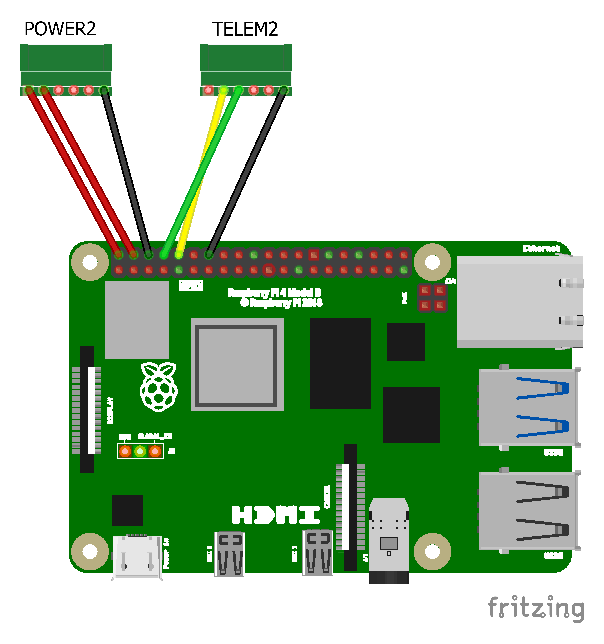
\includegraphics[keepaspectratio]{img/wiring-diagram.pdf}
  \caption{A diagram of the wired connections from the Raspberry Pi 4 to the power management board (TELEM1) and the flight controller (TELEM2).}\label{fig:wiring}
\end{figure}
The second wired connection that needs to be established for this configuration is between the flight controller and the companion computer so the Mavlink messages can be exchanged.
As it is desirable to be able to maintain a wireless link to the vehicle even while it is being controlled by the onboard computer, the telemetry radio is kept connected to the \verb|TELEM1| port of the flight controller and the companion computer is wired to the \verb|TELEM2| port.
This port is not configured to be used by default so it is necessary to modify the configuration of the Pixhawk board either through QGroundControl \todo{More about QGC in SotA} or the PX4 console. \todo{More about this in validation ????}
The other end of the connector has three female Dupont wires that go into the TX/RX UART pins of the Raspberry Pi.
A diagram of the connections to the companion computer can be seen in Figure~\ref{fig:wiring}.
\todo[inline]{Description of 6 wires from connectors both power and telem}

In comparison with the default baudrate of 57600 on the telemetry radio link established in the previous section the wired serial connection works at a baudrate of 921600, which means the data is transferred 16 times faster through the link.
\todo{Main limitation is image processing though, so slower processing power from computer means slower responsiveness to movement all together. Any info about update rate from PX4? Does it depend on the link speed or is it constant?}
\todo[inline]{Link to section in validation where onboard setup is done}

The offboard configuration allowed the supervision of the output from the program while the vehicle was flying, since the computer stayed stationary on the ground, however in this configuration it is not possible to have a screen connected directly to the companion computer.
To fix this situation and be able to monitor during flight, as well as being able to give input directly to the program, it is possible to make use of the WiFi receptor of the Raspberry Pi to configure a remote desktop and connect to it through another computer serving as a ground station;
then the output from the camera and the image recognition can be seen in real time.
A more detailed description of the configuration required can be found on Section~\ref{sec:devenv}.

\begin{figure}
  \centering
  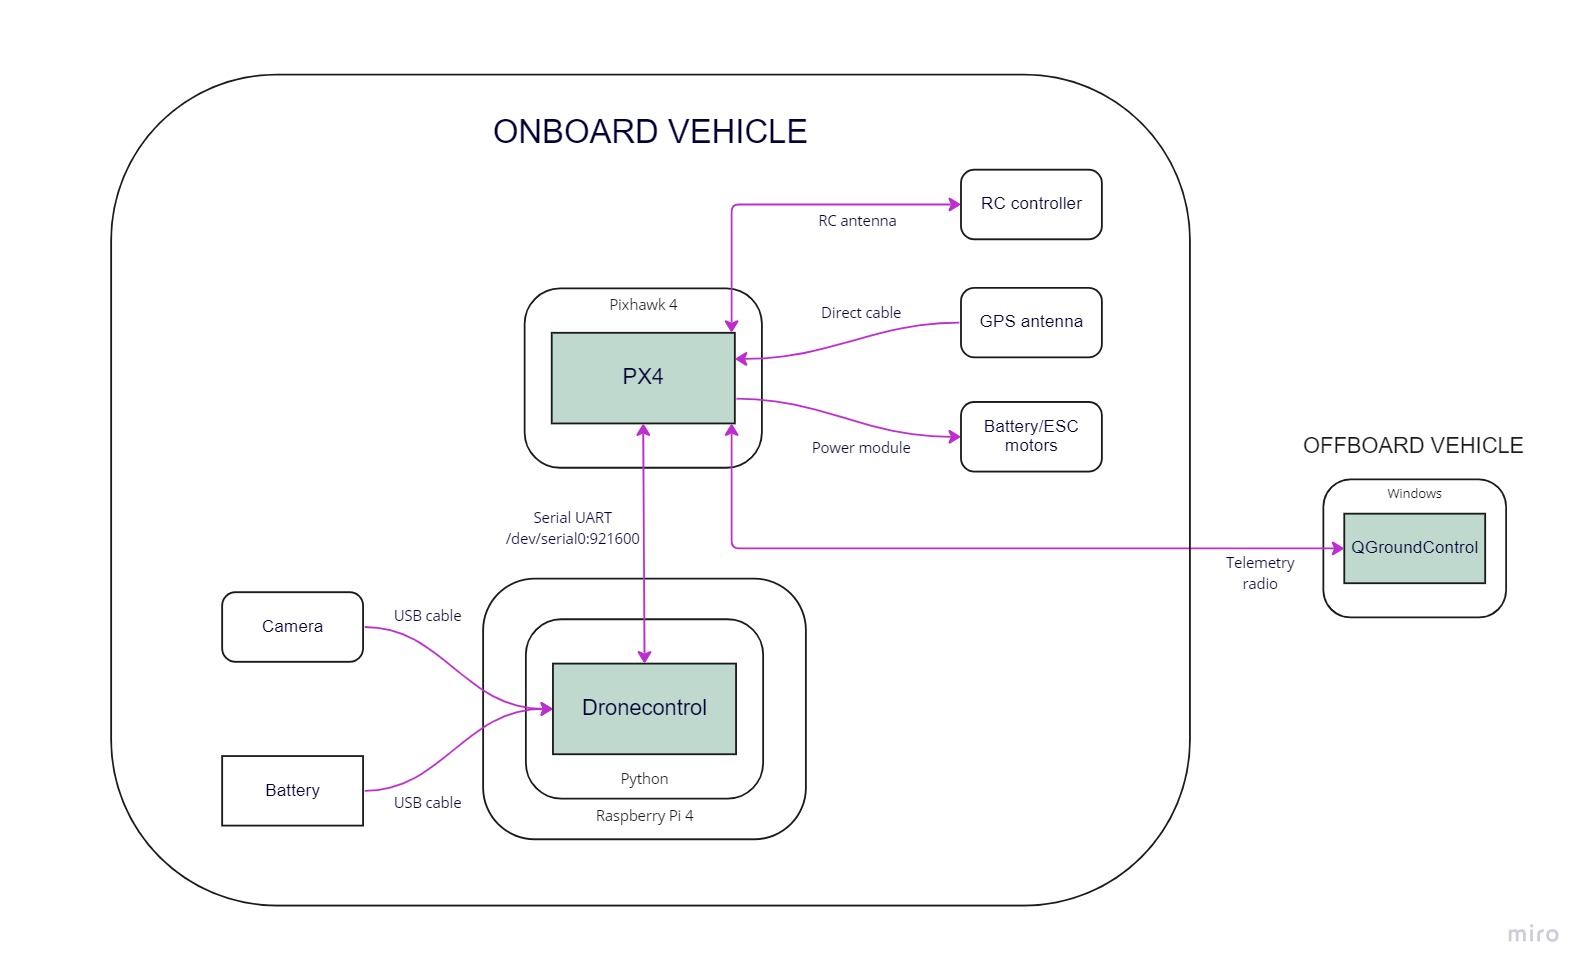
\includegraphics[width=\textwidth,keepaspectratio]{img/onboard-diagram.jpg}
  \caption{Onboard configuration connections}\label{fig:onboard-config}
\end{figure}

